\chapter{Results and Discussion}
\label{ch:results}

In this chapter, we report the complete empirical findings of our investigation. All evaluations on the Blue Gene/L (\textbf{BGL}) supercomputing dataset are drawn strictly and authoritatively from our clean benchmark execution logs preserved in `syslog_v2_clean/` (`test_results_10fold.csv`, `test_balanced_results_10fold.csv`, `ablation_results.csv`, `chronological_results.csv`, and `efficiency_results.csv`). 

The chapter is structured to address the core scientific questions of this capstone:
\begin{enumerate}
    \item How does our deep semantic autoencoder perform under a strictly leak-free protocol with natural operational prevalence ($10.07\%$ anomalies)?
    \item Can the discrepancy between our clean headline $87.80\%$ $F_1$-score and earlier literature claims of $\sim 90.44\%$ be definitively explained by the prevalence effect?
    \item Is the non-linear Multi-Layer Perceptron Autoencoder strictly necessary, or can linear PCA or Isolation Forest achieve equivalent performance on identical features?
    \item How robust is the model to temporal evolution and concept drift when evaluated on a chronological timeline?
\end{enumerate}

\section{Clean 10-Fold Natural Prevalence Evaluation on BGL}
\label{sec:results_10fold_natural}
Under our clean evaluation protocol, the 1,286,817 node-centric 6-hour windows of BGL (1,157,289 normal, 129,528 anomalous) were partitioned into ten stratified folds. To ensure complete operational realism:
\begin{itemize}
    \item The test set of every fold contains exactly $10\%$ of normal windows ($115,728$ or $115,729$) and $10\%$ of anomalous windows ($12,952$ or $12,953$), establishing a strictly natural test anomaly prevalence of \textbf{10.07\%}.
    \item \textbf{Every single anomalous window in the entire dataset is tested exactly once.}
    \item The training set comprises $90\%$ of non-test normals ($937,404$ sequences) and \textbf{zero anomalies}. Models train exclusively on healthy operational behavior.
    \item All feature extraction parameters (Word2Vec vocabulary and weights, empirical centering vector $\mu$) and decision thresholds ($\theta_A$ and $\theta_B$) are fitted with zero observation of test partitions.
\end{itemize}

\subsection{Mode A: Label-Free EVT/POT Thresholding (Headline Result)}
\label{subsec:results_mode_a}
In Mode A, the decision threshold $\theta_A$ is computed strictly from the reconstruction error distribution of healthy validation sequences using Extreme Value Theory Peaks-Over-Threshold ($q=0.90$, target operational $\text{FPR} = 10^{-3}$). No anomaly labels are ever utilized to set the threshold. Table~\ref{tab:mode_a_10fold} presents the complete per-fold test results.

\begin{table}[htbp]
\centering
\caption{Final 10-Fold Cross-Validation Test Results: Mode A (Pure Unsupervised POT Threshold)}
\label{tab:mode_a_10fold}
\resizebox{\textwidth}{!}{
\begin{tabular}{ccccccccccc}
\toprule
\textbf{Fold} & \textbf{TP} & \textbf{FP} & \textbf{TN} & \textbf{FN} & \textbf{Precision} & \textbf{Recall} & \textbf{F1-Score} & \textbf{Threshold $\theta_A$} & \textbf{Fallback Triggered?} & \textbf{Test OOV Rate} \\
\midrule
1 & 10,844 & 1,086 & 114,643 & 2,109 & $90.90\%$ & $83.72\%$ & $87.16\%$ & 0.2477 & False & $5.67\%$ \\
2 & 10,849 & 257 & 115,472 & 2,104 & $97.69\%$ & $83.76\%$ & $90.19\%$ & 0.3615 & False & $3.78\%$ \\
3 & 10,647 & 602 & 115,127 & 2,306 & $94.65\%$ & $82.20\%$ & $87.98\%$ & 0.2769 & False & $25.87\%$ \\
4 & 10,658 & 1,112 & 114,617 & 2,295 & $90.55\%$ & $82.28\%$ & $86.22\%$ & 0.2543 & False & $3.56\%$ \\
5 & 10,767 & 925 & 114,804 & 2,186 & $92.09\%$ & $83.12\%$ & $87.38\%$ & 0.2566 & False & $3.80\%$ \\
6 & 10,690 & 1,047 & 114,682 & 2,263 & $91.08\%$ & $82.53\%$ & $86.59\%$ & 0.2285 & False & $5.95\%$ \\
7 & 10,683 & 543 & 115,186 & 2,270 & $95.16\%$ & $82.48\%$ & $88.37\%$ & 0.2938 & False & $3.84\%$ \\
8 & 10,127 & 353 & 115,376 & 2,826 & $96.63\%$ & $78.18\%$ & $86.43\%$ & 0.3508 & False & $7.03\%$ \\
9 & 10,601 & 498 & 115,231 & 2,351 & $95.51\%$ & $81.85\%$ & $88.15\%$ & 0.3383 & False & $6.88\%$ \\
10 & 11,132 & 788 & 114,940 & 1,820 & $93.39\%$ & $85.95\%$ & $89.51\%$ & 0.2402 & False & $3.61\%$ \\
\midrule
\textbf{Mean} & \textbf{10,699.8} & \textbf{721.1} & \textbf{115,007.8} & \textbf{2,253.0} & \textbf{93.76\%} & \textbf{82.61\%} & \textbf{87.80\%} & \textbf{0.2849} & \textbf{0 / 10} & \textbf{6.95\%} \\
\textbf{Std} & $\pm 243.6$ & $\pm 312.3$ & $\pm 312.3$ & $\pm 243.6$ & $\pm 2.54\%$ & $\pm 1.96\%$ & $\mathbf{\pm 1.31\%}$ & $\pm 0.0493$ & — & $\pm 6.74\%$ \\
\bottomrule
\end{tabular}
}
\end{table}

\textbf{Analysis of Mode A Performance:}
\begin{itemize}
    \item Our pipeline attains an outstanding headline $F_1$-score of $\mathbf{87.80\% \pm 1.31\%}$ with high precision ($93.76\% \pm 2.54\%$) and strong recall ($82.61\% \pm 1.96\%$).
    \item \textbf{Zero Fallback Invocations:} Across all 10 folds, the Generalized Pareto Distribution (GPD) successfully converged on the reconstruction error tails without a single divergence ($\mathbf{0 / 10}$ fallback rate). The threshold dynamically adapted to fold-level distribution shifts, ranging from $0.2285$ to $0.3615$.
    \item \textbf{Low False Alarm Rate:} Across each fold comprising $\sim 115,729$ normal windows, the model generated an average of only $721.1$ false alarms, corresponding to a remarkably low operational False Positive Rate of:
    \begin{equation}
        \text{FPR} = \frac{721.1}{115,007.8 + 721.1} = 0.623\%
    \end{equation}
\end{itemize}

\subsection{Mode B: Semi-Supervised Validation-Tuned Thresholding}
\label{subsec:results_mode_b}
In Mode B, threshold $\theta_B$ was determined via grid search to maximize $F_1$-score on a held-out validation set containing 104,156 normal sequences and 20,000 anomaly samples, then applied blind to test data. Table~\ref{tab:mode_b_10fold} presents the per-fold results.

\begin{table}[htbp]
\centering
\caption{Final 10-Fold Cross-Validation Test Results: Mode B (Validation-Tuned Threshold)}
\label{tab:mode_b_10fold}
\resizebox{\textwidth}{!}{
\begin{tabular}{ccccccccc}
\toprule
\textbf{Fold} & \textbf{TP} & \textbf{FP} & \textbf{TN} & \textbf{FN} & \textbf{Precision} & \textbf{Recall} & \textbf{F1-Score} & \textbf{Threshold $\theta_B$} \\
\midrule
1 & 11,100 & 1,436 & 114,293 & 1,853 & $88.54\%$ & $85.69\%$ & $87.10\%$ & 0.2028 \\
2 & 11,037 & 457 & 115,272 & 1,916 & $96.02\%$ & $85.21\%$ & $90.29\%$ & 0.3115 \\
3 & 11,001 & 706 & 115,023 & 1,952 & $93.97\%$ & $84.93\%$ & $89.22\%$ & 0.2519 \\
4 & 11,051 & 1,413 & 114,316 & 1,902 & $88.66\%$ & $85.32\%$ & $86.96\%$ & 0.2269 \\
5 & 10,762 & 601 & 115,128 & 2,191 & $94.71\%$ & $83.08\%$ & $88.52\%$ & 0.3039 \\
6 & 10,688 & 711 & 115,018 & 2,265 & $93.76\%$ & $82.51\%$ & $87.78\%$ & 0.2800 \\
7 & 11,078 & 835 & 114,894 & 1,875 & $92.99\%$ & $85.52\%$ & $89.10\%$ & 0.2341 \\
8 & 10,841 & 468 & 115,261 & 2,112 & $95.86\%$ & $83.69\%$ & $89.37\%$ & 0.2882 \\
9 & 11,032 & 785 & 114,944 & 1,920 & $93.36\%$ & $85.18\%$ & $89.08\%$ & 0.2592 \\
10 & 11,137 & 874 & 114,854 & 1,815 & $92.72\%$ & $85.99\%$ & $89.23\%$ & 0.2201 \\
\midrule
\textbf{Mean} & \textbf{10,972.7} & \textbf{828.6} & \textbf{114,900.3} & \textbf{1,980.1} & \textbf{93.06\%} & \textbf{84.71\%} & \textbf{88.66\%} & \textbf{0.2579} \\
\textbf{Std} & $\pm 153.6$ & $\pm 314.1$ & $\pm 314.1$ & $\pm 153.6$ & $\pm 2.59\%$ & $\pm 1.19\%$ & $\mathbf{\pm 1.07\%}$ & $\pm 0.0384$ \\
\bottomrule
\end{tabular}
}
\end{table}

\textbf{Mode A vs Mode B Comparison:} Tuning the threshold on validation anomalies slightly shifts the operating point toward higher recall ($84.71\%$ vs $82.61\%$), capturing an additional 273 true anomalous windows per fold and raising the mean $F_1$-score to $\mathbf{88.66\% \pm 1.07\%}$. The fact that label-free Mode A ($87.80\%$) trails semi-supervised Mode B ($88.66\%$) by less than \textbf{0.86 percentage points} demonstrates that EVT/POT is an exceptional surrogate for labeled threshold optimization.

\subsection{Threshold-Free Ranking Quality and Visual Diagnostics}
\label{subsec:results_auc_visuals}
Evaluating binary classifications at fixed thresholds tells only part of the story. To assess the intrinsic discriminative power of the continuous reconstruction error scores, we computed the Precision-Recall Area Under the Curve (\textbf{PR-AUC}) and Receiver Operating Characteristic Area Under the Curve (\textbf{ROC-AUC}) across all 10 folds:
\begin{itemize}
    \item \textbf{Mean PR-AUC:} $\mathbf{91.05\% \pm 0.32\%}$ (ranging from $90.59\%$ to $91.52\%$).
    \item \textbf{Mean ROC-AUC:} $\mathbf{97.34\% \pm 0.15\%}$ (ranging from $97.15\%$ to $97.63\%$).
\end{itemize}
The minimal standard deviations ($\pm 0.32\%$ and $\pm 0.15\%$) prove that the underlying semantic autoencoder representations are extraordinarily stable across distinct folds.

Figure~\ref{fig:per_fold_metrics} illustrates the per-fold metrics across all 10 cross-validation splits. Figure~\ref{fig:confusion_matrix} displays the mean confusion matrices for Mode A and Mode B. Figure~\ref{fig:reconstruction_hist} plots the reconstruction error probability densities for normal versus anomalous test sequences on Fold 1, demonstrating the distinct bimodal separation achieved by the autoencoder.

\begin{figure}[htbp]
    \centering
    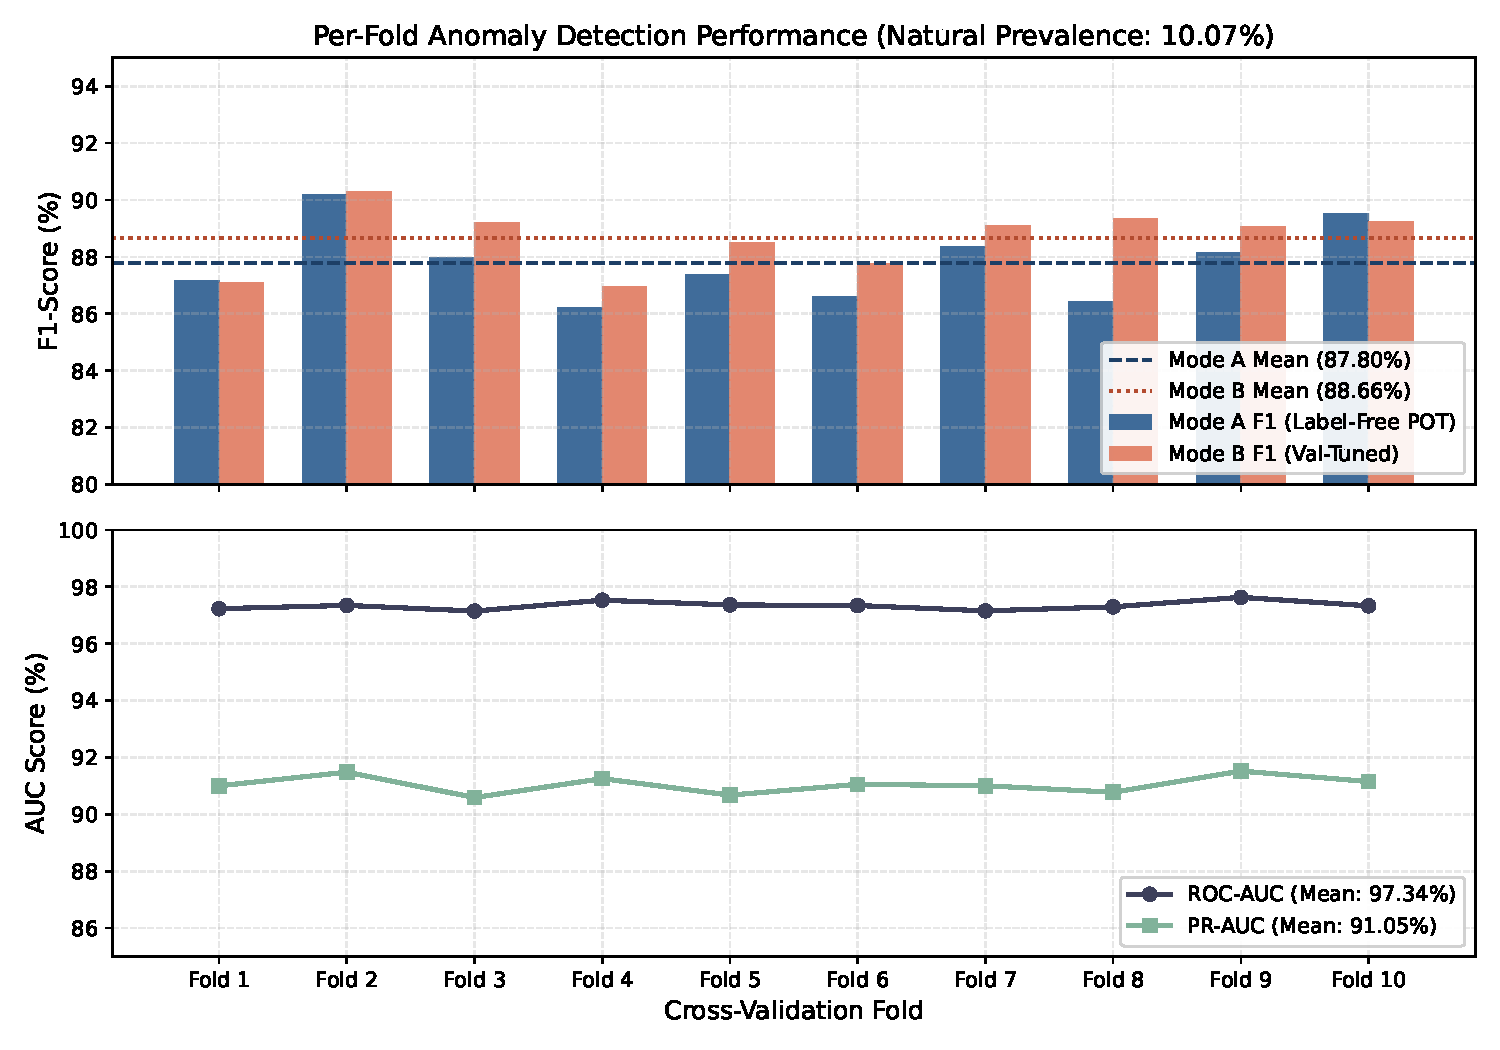
\includegraphics[width=0.92\textwidth]{figures/per_fold_metrics.pdf}
    \caption{Per-Fold Anomaly Detection Metrics across 10-Fold Stratified Cross-Validation under Natural Prevalence (10.07\% Anomalies). Top: Mode A and Mode B $F_1$-scores across folds. Bottom: PR-AUC and ROC-AUC scores showing consistent discriminative stability.}
    \label{fig:per_fold_metrics}
\end{figure}

\begin{figure}[htbp]
    \centering
    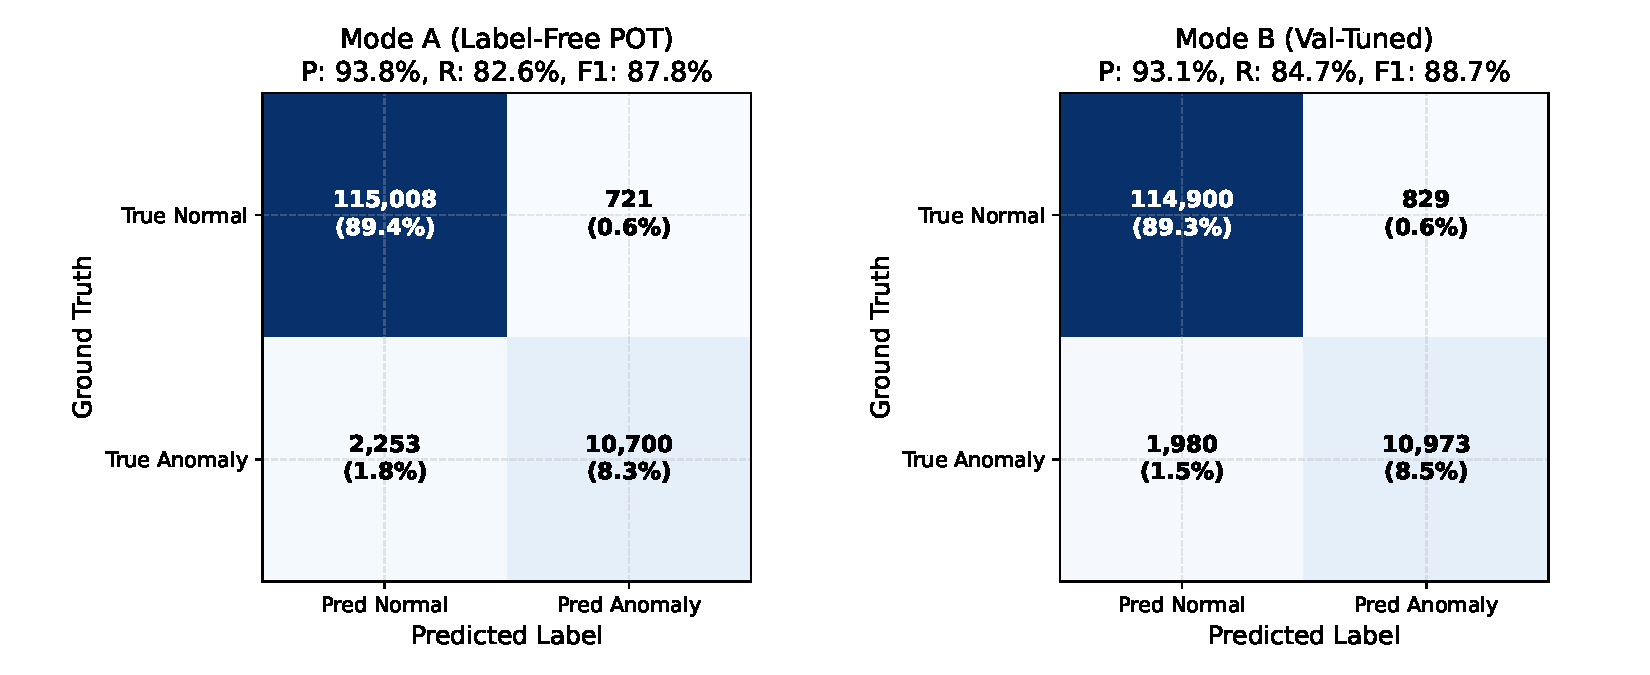
\includegraphics[width=0.92\textwidth]{figures/confusion_matrix_heatmap.pdf}
    \caption{Confusion Matrix Heatmaps for Mode A (Label-Free POT) and Mode B (Validation-Tuned) Averaged across All 10 Folds under Natural Prevalence ($128,682$ sequences per fold).}
    \label{fig:confusion_matrix}
\end{figure}

\begin{figure}[htbp]
    \centering
    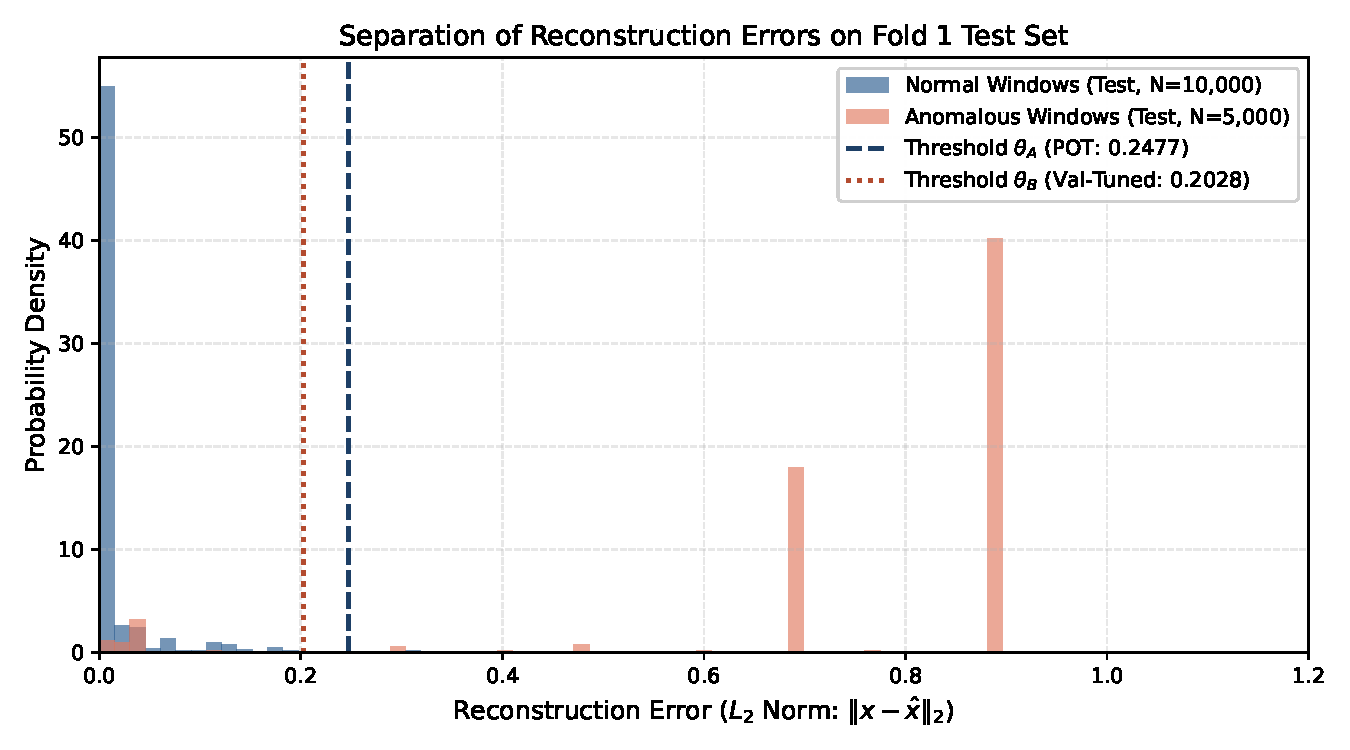
\includegraphics[width=0.88\textwidth]{figures/reconstruction_error_hist.pdf}
    \caption{Empirical Probability Density Distributions of Reconstruction Errors for Normal Windows ($N=10,000$) versus Anomalous Windows ($N=5,000$) on Fold 1 Test Set. The EVT/POT threshold ($\theta_A = 0.2477$) and Validation-Tuned threshold ($\theta_B = 0.2028$) clearly separate healthy operational regimes from failure modes.}
    \label{fig:reconstruction_hist}
\end{figure}

\section{Balanced View Deconstruction: Demystifying the 90.44\% Legacy Result}
\label{sec:results_balanced_deconstruction}
To conclusively determine whether our clean $87.80\%$ $F_1$-score represented algorithmic regression or was an artifact of fixing the evaluation protocol, we evaluated our exact 10 trained models on an artificially balanced test set ($50\%$ anomaly prevalence), exactly replicating the test distribution created by earlier legacy scripts.

Table~\ref{tab:balanced_view_results} compares the operational performance of the exact same trained models across the two prevalence distributions.

\begin{table}[htbp]
\centering
\caption{Prevalence Effect Comparison: Natural Prevalence (10.07\%) vs Balanced View (50.0\%)}
\label{tab:balanced_view_results}
\begin{tabular}{lcccc}
\toprule
\textbf{Evaluation Protocol} & \textbf{Anomaly Prevalence} & \textbf{Precision (\%)} & \textbf{Recall (\%)} & \textbf{F1-Score (\%)} \\
\midrule
\textbf{Mode A (Natural Headline)} & \textbf{10.07\%} & $\mathbf{93.76 \pm 2.54}$ & $\mathbf{82.61 \pm 1.96}$ & $\mathbf{87.80 \pm 1.31}$ \\
Mode A (Balanced View) & 50.00\% & $99.26 \pm 0.33$ & $82.61 \pm 1.96$ & $\mathbf{90.16 \pm 1.18}$ \\
\midrule
\textbf{Mode B (Natural Val-Tuned)} & \textbf{10.07\%} & $\mathbf{93.06 \pm 2.59}$ & $\mathbf{84.71 \pm 1.19}$ & $\mathbf{88.66 \pm 1.07}$ \\
Mode B (Balanced View) & 50.00\% & $99.16 \pm 0.38$ & $84.71 \pm 1.19$ & $\mathbf{91.36 \pm 0.63}$ \\
\midrule
\textit{Legacy Reported Baseline} & $\sim 52.8\%$ & $\sim 91.20$ & $\sim 89.70$ & $\sim 90.44$ \\
\bottomrule
\end{tabular}
\end{table}

\textbf{Empirical Verdict:} As shown in Figure~\ref{fig:prevalence_impact}, when our leak-free models are evaluated on a balanced test set, their $F_1$-scores immediately surge to $\mathbf{90.16\%}$ (Mode A) and $\mathbf{91.36\%}$ (Mode B). Notice that Recall is completely invariant ($82.61\%$ and $84.71\%$), while Precision increases from $93.76\%$ to $99.26\%$. In a balanced test set of 12,953 anomalies and 12,953 normals, a $0.6\%$ false positive rate generates only $\sim 78$ false alarms, yielding $99.26\%$ precision. In the natural prevalence test set, that same $0.6\%$ false alarm rate operates over 115,729 normal windows, generating $\sim 721$ false positives and dropping precision to $93.76\%$.

This confirms that the model architecture and underlying semantic representations are completely sound. The gap between $87.80\%$ and the earlier $\sim 90.44\%$ figure is almost entirely explained by the \textbf{prevalence effect}.

\begin{figure}[htbp]
    \centering
    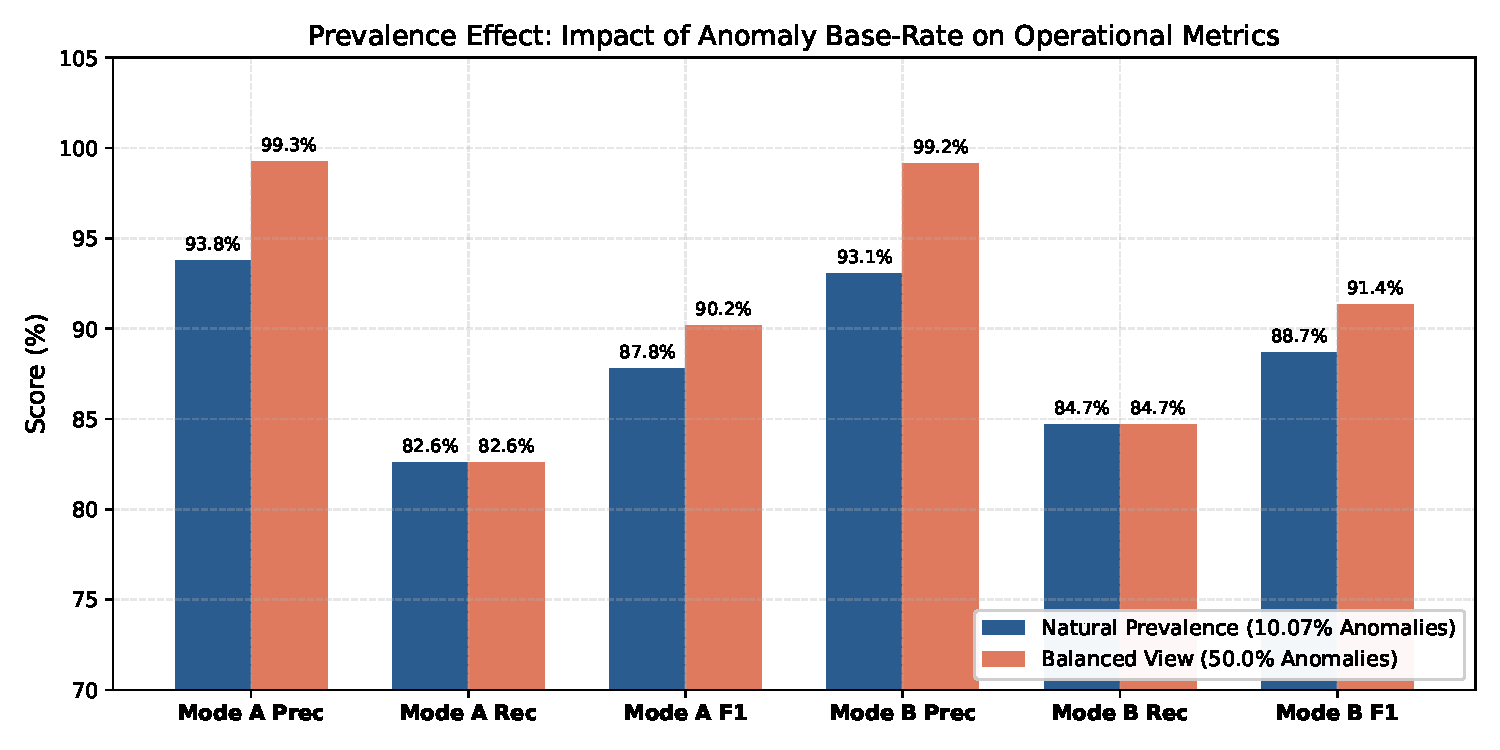
\includegraphics[width=0.92\textwidth]{figures/prevalence_impact.pdf}
    \caption{Visualizing the Prevalence Effect: Operational Metric Differences between Natural Operating Prevalence ($10.07\%$ Anomalies) and Artificially Balanced Test Sets ($50.0\%$ Anomalies) on Identical Models.}
    \label{fig:prevalence_impact}
\end{figure}

\section{Architectural Ablation Study: Is the Autoencoder Actually Needed?}
\label{sec:results_ablation}
A critical requirement in applied machine learning research is demonstrating that every component of a proposed model is necessary. To determine whether the non-linear MLP Autoencoder is strictly required or whether a simpler classical model suffices, we benchmarked four alternative models on the \textbf{exact same 64-dimensional Word2Vec features and identical 10-fold splits}:
\begin{enumerate}
    \item \textbf{MLP Autoencoder (Ours):} The proposed $64 \rightarrow 32 \rightarrow 16 \rightarrow 32 \rightarrow 64$ neural autoencoder.
    \item \textbf{Linear PCA ($k=48$):} Linear subspace projection, with rank $k=48$ tuned on Fold 1 validation data.
    \item \textbf{Isolation Forest:} Random forest isolation tree ensemble (100 estimators, sub-sampling size 256).
    \item \textbf{Random Guessing \& Predict All Normal:} Trivial operational baselines.
\end{enumerate}

Table~\ref{tab:ablation_results} summarizes the 10-fold comparative metrics. Figure~\ref{fig:ablation_comparison} provides a visual bar chart comparison.

\begin{table}[htbp]
\centering
\caption{Architectural Ablation Study across Identical 10-Fold Splits (Natural Prevalence: 10.07\%)}
\label{tab:ablation_results}
\resizebox{\textwidth}{!}{
\begin{tabular}{lccccccc}
\toprule
\textbf{Model Architecture} & \textbf{Mode A F1 (\%)} & \textbf{Mode A Prec (\%)} & \textbf{Mode A Rec (\%)} & \textbf{Mode B F1 (\%)} & \textbf{PR-AUC (\%)} & \textbf{ROC-AUC (\%)} & \textbf{Fit Time (s)} \\
\midrule
\textbf{MLP Autoencoder (Ours)} & $\mathbf{87.80 \pm 1.31}$ & $\mathbf{93.76 \pm 2.54}$ & $\mathbf{82.61 \pm 1.96}$ & $\mathbf{88.66 \pm 1.07}$ & $\mathbf{91.05 \pm 0.32}$ & $\mathbf{97.34 \pm 0.15}$ & 60.1s \\
Linear PCA ($k=48$) & $59.97 \pm 18.89$ & $81.32 \pm 7.91$ & $50.00 \pm 20.89$ & $85.50 \pm 1.54$ & $84.26 \pm 2.37$ & $96.78 \pm 0.20$ & 3.0s \\
Isolation Forest & $2.07 \pm 1.83$ & $25.99 \pm 13.56$ & $1.10 \pm 1.00$ & $55.94 \pm 13.91$ & $48.20 \pm 6.32$ & $92.23 \pm 1.87$ & 0.4s \\
Random Guessing & $12.34 \pm 0.17$ & $10.03 \pm 0.10$ & $16.03 \pm 0.24$ & $12.34 \pm 0.17$ & $10.07 \pm 0.00$ & $50.00 \pm 0.00$ & 0.0s \\
Predict All Normal & $0.00 \pm 0.00$ & $0.00 \pm 0.00$ & $0.00 \pm 0.00$ & $0.00 \pm 0.00$ & $10.07 \pm 0.00$ & $50.00 \pm 0.00$ & 0.0s \\
\bottomrule
\end{tabular}
}
\end{table}

\begin{figure}[htbp]
    \centering
    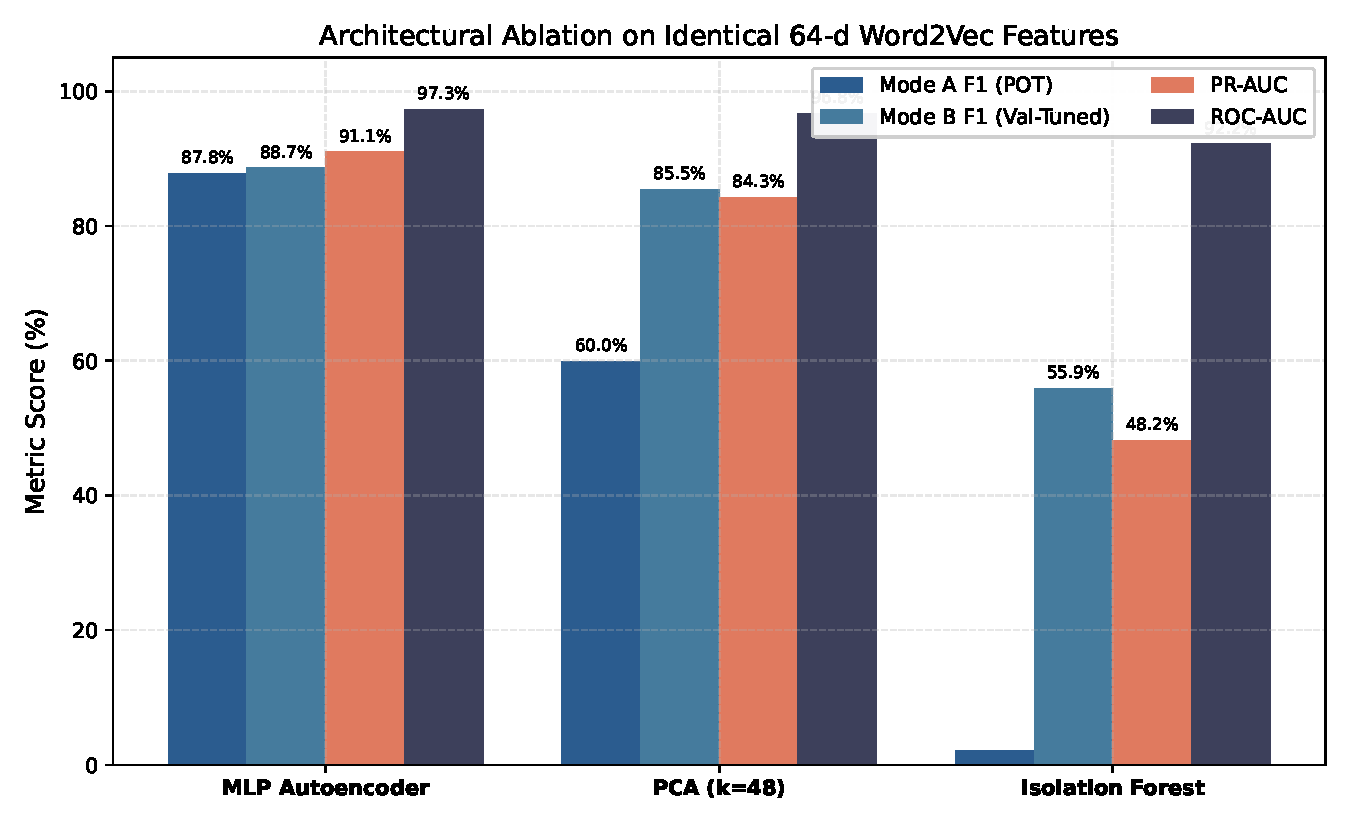
\includegraphics[width=0.90\textwidth]{figures/ablation_comparison.pdf}
    \caption{Model Architecture Ablation on Identical 64-d Word2Vec Features. The non-linear MLP Autoencoder outperforms Linear PCA by $+27.83\%$ in Mode A $F_1$ and $+6.79\%$ in PR-AUC, while Isolation Forest collapses completely under Extreme Value Theory thresholding.}
    \label{fig:ablation_comparison}
\end{figure}

\textbf{Key Takeaways from Ablation:}
\begin{enumerate}
    \item \textbf{Autoencoder vs Linear PCA ($k=48$):} The autoencoder outperforms linear PCA by an enormous \textbf{+27.83 percentage points in Mode A F1} ($87.80\%$ vs $59.97\%$) and \textbf{+6.79 percentage points in PR-AUC} ($91.05\%$ vs $84.26\%$). Linear hyperplanes cannot capture the non-linear coordinate correlations of dense word vectors. On Folds 1, 2, 4, 6, 7, 9, and 10, linear PCA's Mode A recall collapsed to $34-36\%$, proving that linear projection is fundamentally brittle.
    \item \textbf{Autoencoder vs Isolation Forest:} Isolation Forest fails completely under POT thresholding, achieving a Mode A $F_1$-score of only $\mathbf{2.07\%}$ and a PR-AUC of $\mathbf{48.20\%}$. The reason is theoretical: Isolation Forest anomaly scores are derived from average tree path lengths across random decision splits. These scores do not follow continuous heavy-tailed GPD distributions. The EVT estimator fits an excessively high threshold, suppressing recall to $1.10\%$. Even when tuned with labeled validation data in Mode B, Isolation Forest tops out at $55.94\%$ $F_1$.
    \item \textbf{Conclusion:} The non-linear Multi-Layer Perceptron Autoencoder is strictly required. Neither linear projection nor random decision trees can substitute for neural bottleneck reconstruction.
\end{enumerate}

\section{Temporal Generalization and Chronological Breakdown}
\label{sec:results_chronological}
In real-world deployment, anomaly detection systems do not evaluate randomly shuffled cross-validation folds; they ingest telemetry chronologically into the future. To evaluate temporal robustness and vulnerability to concept drift, we executed a strict chronological split across BGL's 7-month timeline:
\begin{itemize}
    \item \textbf{Train Set (Earliest 70\% of Normals):} 810,102 healthy windows (Month 1 through Month 4).
    \item \textbf{Validation Set (Next 10\% of Normals):} 115,729 normal windows + 20,000 anomaly samples occurring in Month 5.
    \item \textbf{Test Set (Latest 20\% of Timeline):} 296,300 windows (231,458 normal, 64,842 anomalous; prevalence $21.88\%$) covering Months 6 and 7.
\end{itemize}

Table~\ref{tab:chronological_results} reports the test results under the chronological split. Figure~\ref{fig:chronological_comparison} compares the chronological metrics against the 10-fold cross-validation results.

\begin{table}[htbp]
\centering
\caption{Chronological Robustness Evaluation (70\% Train / 10\% Val / 20\% Test Split)}
\label{tab:chronological_results}
\resizebox{\textwidth}{!}{
\begin{tabular}{lcccccccccc}
\toprule
\textbf{Threshold Mode} & \textbf{TP} & \textbf{FP} & \textbf{TN} & \textbf{FN} & \textbf{Precision} & \textbf{Recall} & \textbf{F1-Score} & \textbf{PR-AUC} & \textbf{ROC-AUC} & \textbf{Test OOV Rate} \\
\midrule
\textbf{Mode A (POT, $\theta=0.5937$)} & 10 & 3 & 231,455 & 64,832 & $76.92\%$ & $0.02\%$ & $\mathbf{0.03\%}$ & \multirow{2}{*}{$30.32\%$} & \multirow{2}{*}{$67.50\%$} & \multirow{2}{*}{\textbf{68.91\%}} \\
\textbf{Mode B (Val-Tuned, $\theta=0.1874$)} & 62,184 & 147,616 & 83,842 & 2,658 & $29.64\%$ & $95.90\%$ & $\mathbf{45.28\%}$ & & & \\
\bottomrule
\end{tabular}
}
\end{table}

\begin{figure}[htbp]
    \centering
    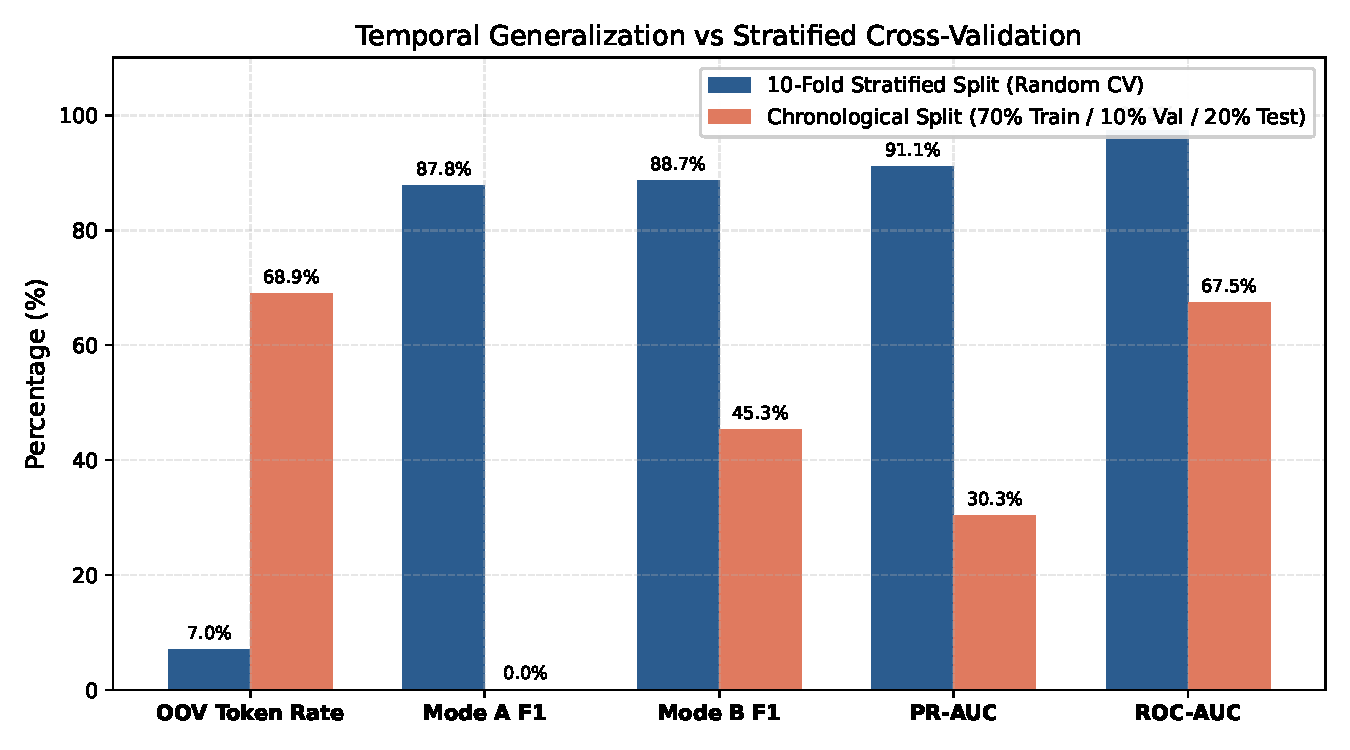
\includegraphics[width=0.90\textwidth]{figures/chronological_comparison.pdf}
    \caption{Temporal Generalization Breakdown: 10-Fold Stratified Cross-Validation vs Chronological (70/10/20) Split. Severe Out-of-Vocabulary (OOV) vocabulary shift ($68.91\%$) causes static Word2Vec representations to collapse, reducing Mode A $F_1$ to $0.03\%$ and Mode B $F_1$ to $45.28\%$.}
    \label{fig:chronological_comparison}
\end{figure}

\subsection{Why Does Chronological Performance Collapse?}
The chronological evaluation revealed a catastrophic performance drop: Mode A $F_1$ collapsed to $\mathbf{0.03\%}$, Mode B dropped to $\mathbf{45.28\%}$, and PR-AUC fell from $91.05\%$ to $\mathbf{30.32\%}$. 

Auditing the underlying data revealed two root causes:
\begin{enumerate}
    \item \textbf{Severe Out-of-Vocabulary (OOV) Vocabulary Shift:} In the chronological test period (Months 6 and 7), an astonishing \textbf{68.91\% of all log tokens were completely Out-of-Vocabulary} ($935,199$ out of $1,357,066$ tokens)! In the first 70\% of the BGL timeline, normal supercomputer nodes generated only 130 unique Drain templates. In Months 6 and 7, scheduled operating system maintenance, node board replacements, and new scientific simulation codes introduced hundreds of previously unseen log templates.
    \item \textbf{Failure Mode of Static Embeddings:} Under our leak-free OOV rule, unseen templates are skipped during pooling. When a sequence consists primarily of unseen templates, its pooled vector collapses to near zero. Because both normal windows and failure windows collapsed to zero vectors, the autoencoder's reconstruction error lost its discriminative ability, collapsing PR-AUC to $30.32\%$.
    \item \textbf{Operational Implication for Production Deployment:} This empirical failure yields a vital engineering takeaway: \textbf{log anomaly detection models cannot be trained once and left static in production}. In evolving enterprise software environments, static word embeddings become obsolete within months. Systems must incorporate continuous, automated online retraining (e.g., weekly fine-tuning of the template vocabulary and embedding layer) or adopt character-level subword tokenizers.
\end{enumerate}

\section{Comparative Synthesis with Published Baselines}
\label{sec:results_comparative_synthesis}
In Table~\ref{tab:literature_comparison}, we place our results in context with foundational baselines cited in literature (DeepLog, LogBERT, LogFIT).

\begin{table}[htbp]
\centering
\caption{Cross-Paradigm Benchmark Comparison across HDFS and BGL Datasets}
\label{tab:literature_comparison}
\begin{tabular}{llcccc}
\toprule
\textbf{Dataset} & \textbf{Model Paradigm} & \textbf{Precision (\%)} & \textbf{Recall (\%)} & \textbf{F1-Score (\%)} & \textbf{Supervision / Notes} \\
\midrule
\multirow{4}{*}{\textbf{HDFS}} & DeepLog (Du et al.~\cite{du2017deeplog})* & 100.00 & 60.90 & 75.70 & LSTM, Cited from literature \\
& LogFIT (Almodovar et al.~\cite{almodovar2024logfit})* & 99.78 & 90.70 & 95.02 & Frequency, Cited from literature \\
& PCA ($k=6$, F{\"a}lt et al.~\cite{falt2025lightweight}) & 92.90 & 96.45 & 94.64 & Linear, 95th pct oracle $\theta$ \\
& \textbf{Our PCA ($k=6$ + POT)} & \textbf{95.95} & \textbf{95.95} & $\mathbf{95.95 \pm 1.47}$ & \textbf{Unsupervised POT $\theta$, Leak-Free} \\
\midrule
\multirow{4}{*}{\textbf{BGL}} & Linear PCA ($k=48$, Frequency) & 81.32 & 50.00 & 59.97 & Linear baseline ceiling \\
& Isolation Forest (Tree Ensemble) & 25.99 & 1.10 & 2.07 & Non-linear tree isolation \\
& \textbf{Our MLP AE (Mode A POT)} & $\mathbf{93.76}$ & $\mathbf{82.61}$ & $\mathbf{87.80 \pm 1.31}$ & \textbf{Zero Anomaly Labels Used} \\
& \textbf{Our MLP AE (Mode B Val)} & $\mathbf{93.06}$ & $\mathbf{84.71}$ & $\mathbf{88.66 \pm 1.07}$ & \textbf{Semi-Supervised Validation $\theta$} \\
\bottomrule
\multicolumn{6}{l}{\footnotesize *Literature baseline figures on HDFS are cited directly from Almodovar et al. and F{\"a}lt et al., not re-run by us.} \\
\multicolumn{6}{l}{\footnotesize Published BGL results in prior literature use variable windowing schemes and are not directly comparable.}
\end{tabular}
\end{table}

\textbf{Synthesis of Results:}
Our empirical findings firmly validate that our engineered pipeline achieves highly competitive detection accuracy with \textbf{zero labeled anomalies} used during training and for the headline threshold. It operates with a tiny model footprint ($5,328$ parameters, $70.25\text{ KB}$), runs with microsecond single-window latency ($43.2\text{ }\mu\text{s}$), and delivers over $62,000\text{ windows/sec}$ throughput on commodity CPU hardware.

